\documentclass[journal=jpclcd,manuscript=article]{achemso}
\usepackage[version=3]{mhchem}
\usepackage{amsmath}
\usepackage{siunitx}
\usepackage{booktabs}
\usepackage{graphicx}
\usepackage{caption}

\author{CoChem Research Group}
\affiliation{CoChem Computational Chemistry and Rotational Spectroscopy Campaign}
\email{corresponding@cochem.org}

\title{Comprehensive Computational Materials and Methods: $\ce{HCOOH\bond{...}H2S}$ (SR3) and $\ce{HCOOH\bond{...}N2O}$ (SR4) Campaigns}

\begin{document}

\section{Computational Materials and Methods}

This monograph provides the complete computational materials, algorithmic architecture, mathematical equations, convergence thresholds, hardware queue orchestration, and literature references for the binary formic acid--hydrogen sulfide ($\ce{HCOOH\bond{...}H2S}$, Project SR3) and formic acid--nitrous oxide ($\ce{HCOOH\bond{...}N2O}$, Project SR4) research campaigns \cite{Neese2020, Neese2022, Sun2018, Sun2020, Wu2024, Li2024, Larsen2017, Lu2012, Lu2024}. All calculations were executed through a deterministic, checksum-verified multi-tier funnel:
\begin{align*}
  &\text{Tier 1: Global Exploration (\texttt{GOAT/GFN2-xTB} + 1200-Start Batched GPU \texttt{MACE-OFF24(M)})} \\
  &\quad\longrightarrow\ \text{Tier 2A (GPU-First Basin Filter): \texttt{GPU4PySCF} }\omega\text{B97X-V/def2-TZVPP (or }\omega\text{B97M-V/def2-TZVPPD) Opt + Analytic Hessian} \\
  &\quad\longrightarrow\ \text{Tier 2B (Concurrent CPU Validation): \texttt{r2SCAN-3c} TightOpt + Freq \& 6-Model ML/FF Benchmark} \\
  &\quad\longrightarrow\ \text{Tier 3: \texttt{revDSD-PBEP86-D4/jun-cc-pV(T+d)Z} + \texttt{GPU4PySCF} }\omega\text{B97X-V/def2-TZVPP (\& }\omega\text{B97M-V/def2-TZVPPD) \texttt{VPT2}} \\
  &\quad\longrightarrow\ \text{Tier 4: \texttt{DLPNO-CCSD(T1)/CBS(3/4)} + \texttt{DLPNO-SE} }(R_e^{\mathrm{SE}}, B_e^\alpha) + \texttt{LED} + \texttt{QTAIM/IGMH} + \text{FTMW Simulation}
\end{align*}

\subsection{1. Hardware Queue Orchestration and Determinism Protocols}
Calculations were distributed across CPU and GPU hardware channels without mutual resource contention:
\begin{enumerate}
  \item \textbf{Single-Instance ORCA CPU Serialization (\texttt{campaign\_queue.py}):} All CPU-bound ORCA 6.1.1 \cite{Neese2020, Neese2022} jobs were dispatched sequentially from priority-ordered JSON specifications (\texttt{\_publication/queue/jobs/*.json}) under a workstation-wide lock (\texttt{\%TEMP\%\textbackslash orca\_one\_job\_at\_a\_time.lock}). Each production calculation was allocated 8 dedicated physical performance cores (\texttt{\%pal nprocs 8 end}, \texttt{\%maxcore 3000}) with process-creation rate guards and execution watchdogs.
  \item \textbf{Independent GPU Execution Channel:} Machine-learning potential relaxations (\texttt{PyTorch}/\texttt{ASE} \cite{Larsen2017}) and range-separated hybrid DFT optimizations (\texttt{GPU4PySCF 1.9.0} \cite{Sun2018, Sun2020, Wu2024, Li2024}) were executed on an NVIDIA GeForce RTX 3090 GPU (24~GB GDDR6X VRAM, CUDA 12) independently of the CPU lock.
  \item \textbf{Deterministic Data Normalization (\texttt{pubstyle.py}):} All intermediate CSV files, Excel workbooks, LaTeX tables, and figures were strictly schema-checked (\texttt{pubstyle.check\_results(..., strict=True)}) to ensure reproducibility and prevent unphysical coordinate or vibrational artifacts.
\end{enumerate}

\subsection{2. Chronological Ten-Tier Computational Methodology}

\subsubsection{2.1. Gas-Phase Monomer Parameters and Reference Geometries}
Experimental monomer structures and spectroscopic constants established the baseline for all complexation properties:
\begin{enumerate}
  \item \textbf{Formic Acid ($\ce{HCOOH}$):} The planar \textit{trans}-rotamer ($\tau(\ce{H-C-O-H}) = 0.0^\circ$) has ground-state rotational constants $A_0 = 77512.28\text{ MHz}$, $B_0 = 12055.10\text{ MHz}$, and $C_0 = 10416.19\text{ MHz}$ and dipole moment $\mu = 1.41\text{ D}$ ($\mu_a = -1.39\text{ D}, \mu_b = +0.26\text{ D}$) \cite{Winnewisser2002}. The higher-energy \textit{cis}-rotamer ($\tau(\ce{H-C-O-H}) = 180.0^\circ$) lies $\Delta E_0 = 3.90\text{ kcal mol}^{-1}$ ($1365\text{ cm}^{-1}$) higher in energy with $A_0 = 69829.1\text{ MHz}$, $B_0 = 12398.9\text{ MHz}$, $C_0 = 10526.4\text{ MHz}$, and dipole moment $\mu = 3.79\text{ D}$ ($\mu_a = -2.71\text{ D}, \mu_b = +2.65\text{ D}$) \cite{Winnewisser2002}.
  \item \textbf{Hydrogen Sulfide ($\ce{H2S}$):} Bent $C_{2v}$ molecule with $r(\ce{S-H}) = 1.336\text{ \AA}$, $\angle(\ce{H-S-H}) = 92.1^\circ$, $A_0 = 310180\text{ MHz}$, $B_0 = 270770\text{ MHz}$, $C_0 = 142700\text{ MHz}$, and dipole moment $\mu = \mu_b = 0.97\text{ D}$. The quadrupolar $^{33}\ce{S}$ nucleus ($I = 3/2$) possesses $Q(^{33}\ce{S}) = -67.8\text{ mb}$ \cite{Pyykko2018}, yielding monomer coupling constants $\chi_{aa} = -32.55\text{ MHz}$, $\chi_{bb} = -8.11\text{ MHz}$, and $\chi_{cc} = +40.66\text{ MHz}$.
  \item \textbf{Nitrous Oxide ($\ce{N2O}$):} Linear triatomic rod ($\ce{N_t\equiv N_c^+-O^-}$) with $r(\ce{N_t-N_c}) = 1.1282\text{ \AA}$, $r(\ce{N_c-O}) = 1.1842\text{ \AA}$, $B_0 = 12561.63\text{ MHz}$, and $\mu = 0.166\text{ D}$. Both nitrogens are quadrupolar $^{14}\ce{N}$ nuclei ($I = 1, Q = +20.44\text{ mb}$ \cite{Pyykko2018}) with distinct monomer coupling constants: $eQq(\ce{N_t}) = -0.7918(5)\text{ MHz}$ and $eQq(\ce{N_c}) = -0.26758(30)\text{ MHz}$ \cite{Pyykko2018, Duarte2017}.
  \item \textbf{Literature Baselines:} For $\ce{HCOOH\bond{...}H2S}$, Kohli and Mittal \cite{Kohli2022} reported 4 \textit{trans}-only MP2/6-311++G(2d,2p) structures without \textit{cis} conformers or rotational constants; experimental analogues include $\ce{HCOOH\bond{...}H2O}$ \cite{Priem2000}, $\ce{HCOOH\bond{...}CO2}$ \cite{Li2015}, $(\ce{H2S})_2$ \cite{Das2018, Biswas2024}, ethylene--$\ce{H2S}$ \cite{Goswami2011}, fenchone--$\ce{H2S}$ \cite{Medcraft2022}, thiophene--$\ce{HCOOH}$ \cite{Obenchain2022}, and furan--$\ce{HCOOH}$ \cite{Evangelisti2013}, alongside broader sulfur noncovalent surveys \cite{Juanes2019}. For $\ce{HCOOH\bond{...}N2O}$, Duarte et al.\ \cite{Duarte2017} characterized four conformers in Ar matrices among 17 theoretical MP2 and \texttt{CCSD(T)-F12a} \cite{Adler2007} structures (\texttt{1t}--\texttt{8t}, \texttt{1c}--\texttt{9c}).
\end{enumerate}

\subsubsection{2.2. Semiempirical Global Conformational Search (\texttt{ORCA GOAT / GFN2-xTB})}
Global conformational exploration was executed using the Global Optimizer Algorithm (\texttt{GOAT}) \cite{deSouza2025} in ORCA 6.1.1 \cite{Neese2020, Neese2022} coupled with \texttt{GFN2-xTB} \cite{Bannwarth2019} (\texttt{! GFN2-xTB GOAT}). Searches were seeded from \textit{trans}-$\ce{HCOOH}$, \textit{cis}-$\ce{HCOOH}$, and \textit{gauche}-$\ce{HCOOH}$ rotamers (\texttt{hcooh-hsh-goat-xtb.py}, \texttt{make\_cis\_gauche\_seeds.py}, \texttt{merge\_isomer\_sets.py}, \texttt{goat\_isomer\_search.py}), yielding 14 candidate conformers for $\ce{HCOOH\bond{...}H2S}$ (\texttt{isomer-00}--\texttt{isomer-13}) and 21 candidates for $\ce{HCOOH\bond{...}N2O}$ (\texttt{isomer-00}--\texttt{isomer-20}), alongside \texttt{GOAT-TS} interconversion transition states.

In $\ce{HCOOH\bond{...}N2O}$, \texttt{GFN2-xTB} exhibited a qualitative inversion of the global minimum, predicting N-bonded \texttt{2t} (\texttt{isomer-00}, $\Delta E_e = 0.000\text{ kcal mol}^{-1}$) to be $0.909\text{ kcal mol}^{-1}$ more stable than the true cyclic O-bonded global minimum \texttt{1t} (\texttt{isomer-01}, $\Delta E_e = +0.909\text{ kcal mol}^{-1}$), inverting the \texttt{CCSD(T)-F12a} ordering of Duarte et al.\ \cite{Duarte2017}.

\subsubsection{2.3. Batched In-Process GPU Machine-Learned Interatomic Potential (\texttt{MACE-OFF24(M)}) Isomer Search and Hierarchical Deduplication (\texttt{mace\_off24m\_isomer\_search.py})}
Coupling ORCA \texttt{GOAT} to external ML potentials via ORCA's \texttt{ExtOpt} interface (\texttt{hcooh-hsh-goat-mace-off24m.py}) incurred $\sim 3.5\text{ s}$ per gradient call due to subprocess spawning overhead ($\sim 97\text{ h}$ projected runtime). We therefore engineered a 7-phase, in-process, GPU-vectorized conformational search and hierarchical deduplication engine (\texttt{mace\_off24m\_isomer\_search.py}) powered by \textbf{\texttt{MACE-OFF24(M)}} \cite{Kovacs2025, Batatia2022} on the RTX 3090 GPU:
\begin{enumerate}
  \item \textbf{Phase 1 (Monomer Reference Relaxation):} Isolated \textit{trans}-$\ce{HCOOH}$, \textit{cis}-$\ce{HCOOH}$, $\ce{H2S}$, and $\ce{N2O}$ monomers were relaxed in \texttt{float64} precision using \texttt{BFGS} in \texttt{ASE} \cite{Larsen2017} ($f_{\max} \le 2.0\times 10^{-4}\text{ eV \AA}^{-1}$), establishing exact reference monomer energies $E_{\mathrm{mon}}$ and equilibrium intramolecular coordinates.
  \item \textbf{Phase 2 (Stratified 5-DOF $\mathrm{SO}(3)\times S^2$ Shell + Sobol Seeding):} Using a deterministic \texttt{PCG64} pseudorandom generator (\texttt{SEED = 20260411}), $1200$ initial dimer placements ($600$ \textit{trans}-$\ce{HCOOH}$ + $600$ \textit{cis}-$\ce{HCOOH}$) were generated per complex ($1204$ total starts in $\ce{HCOOH\bond{...}H2S}$ including $4$ literature/DFT seeds; $1209$ total starts in $\ce{HCOOH\bond{...}N2O}$ including $9$ \texttt{GFN2-xTB} seeds). For each start, the partner molecule ($\ce{H2S}$ or $\ce{N2O}$) was rotated by a Haar-uniform random rotation matrix $\mathbf{R}_{\mathrm{mol}} \in \mathrm{SO}(3)$ (QR decomposition of a $\mathcal{N}(0,1)^{3\times 3}$ matrix with $\det\mathbf{R}_{\mathrm{mol}} = +1$) and placed on a spherical shell around the $\ce{HCOOH}$ center of mass at $R_{\mathrm{COM}} \sim \mathcal{U}(3.0\text{ \AA}, 4.8\text{ \AA})$, rejecting configurations with inter-fragment atomic clashes $d_{ij} < 1.75\text{ \AA}$.
  \item \textbf{Phase 3 (Vectorized \texttt{float32} Batched \texttt{FIRE} Coarse Relaxation):} Rather than relaxing structures sequentially, we constructed a batched \texttt{PyTorch Geometric} graph wrapper (\texttt{BatchedMace}) that packs $B = 256$ independent dimer graphs ($256\times 8 = 2048$ atoms) into a single block-diagonal forward and backward pass on the GPU in \texttt{float32} precision. All $B$ configurations were relaxed simultaneously using a custom vectorized Fast Inertial Relaxation Engine (\texttt{batched\_fire}) \cite{Bitzek2006}:
  \begin{equation}
    \mathbf{v}_b \leftarrow (1 - \alpha_b)\mathbf{v}_b + \alpha_b \frac{\|\mathbf{v}_b\|}{\|\mathbf{F}_b\|}\mathbf{F}_b, \qquad P_b = \mathbf{F}_b \cdot \mathbf{v}_b,
  \end{equation}
  with per-system adaptive velocity damping $\alpha_b$, time-step scaling $\Delta t_b \in [0.02, 0.25]\text{ fs}$ ($f_{\mathrm{inc}} = 1.10, f_{\mathrm{dec}} = 0.50$), maximum atomic displacement step $0.15\text{ \AA}$ per iteration, and harmonic center-of-mass tether $k_{\mathrm{tether}} = 0.50\text{ eV \AA}^{-2}$ for $R_{\mathrm{COM}} > 5.8\text{ \AA}$ ($450$ steps, $f_{\max} \le 5.0\times 10^{-3}\text{ eV \AA}^{-1}$). In $\ce{HCOOH\bond{...}H2S}$, $1192/1204$ ($99.0\%$) starts converged in $11.42\text{ min}$ ($685\text{ s}$, $1.76\text{ starts s}^{-1}$); in $\ce{HCOOH\bond{...}N2O}$, $1120/1209$ ($92.6\%$) starts converged in $14.82\text{ min}$ ($889\text{ s}$, $1.36\text{ starts s}^{-1}$).
  \item \textbf{Phase 4 (Coarse Deduplication \& \texttt{float64} \texttt{BFGS} Tight Refinement):} Coarse endpoints were pre-screened via fast sorted interatomic distance-matrix fingerprints ($\|\mathbf{D}_{\mathrm{sort}}^{(A)} - \mathbf{D}_{\mathrm{sort}}^{(B)}\|_{\max} < 0.12\text{ \AA}$, $\Delta E < 0.08\text{ kcal mol}^{-1}$) and symmetry-aware Kabsch $\mathrm{RMSD} < 0.12\text{ \AA}$, consolidating the $1192$ $\ce{H2S}$ endpoints into $365$ unique coarse basins and the $1120$ $\ce{N2O}$ endpoints into $440$ coarse basins. Each coarse representative was then tightly refined in \texttt{float64} double precision using \texttt{BFGS} ($f_{\max} \le 3.0\times 10^{-4}\text{ eV \AA}^{-1}$, up to $600$ steps; $19.25\text{ min}$ in $\ce{H2S}$ and $36.08\text{ min}$ in $\ce{N2O}$). Dissociated or repulsive structures ($R_{\mathrm{COM}} > 6.0\text{ \AA}$, $d_{\mathrm{inter},\min} > 4.2\text{ \AA}$, or $\Delta E_{\mathrm{bind}} > -0.20\text{ kcal mol}^{-1}$) were discarded.
  \item \textbf{Phase 5 (Hierarchical Geometry-First Symmetry \& Enantiomeric Deduplication):} Tightly converged structures were deduplicated by a two-stage hierarchical clustering algorithm:
  \begin{enumerate}
    \item \textit{Stage A (Fine Duplicate Removal):} Structures were sorted by electronic energy and merged if (a) relative energy agreed within $|\Delta E_i - \Delta E_j| \le 0.05\text{ kcal mol}^{-1}$ and rotational constants plus planar moment $P_{cc}$ agreed within $1.5\%$ ($\le 15\text{ MHz}$) with $\mathrm{RMSD}_{\mathrm{sym}} \le 0.18\text{ \AA}$, or (b) pure permutation- and reflection-invariant Kabsch $\mathrm{RMSD}_{\mathrm{sym}} \le 0.12\text{ \AA}$ \cite{Kabsch1976}:
    \begin{equation}
      \mathrm{RMSD}_{\mathrm{sym}} = \min_{\mathbf{P} \in \mathcal{S}_{\mathrm{ident}}} \min_{\sigma \in \{+1,-1\}} \min_{\mathbf{U} \in \mathrm{SO}(3)} \left( \frac{1}{N}\sum_{i=1}^N \left\|\mathbf{x}_i^{(A)} - \sigma\mathbf{U}\mathbf{x}_{\mathbf{P}(i)}^{(B)}\right\|^2 \right)^{1/2},
    \end{equation}
    where $\sigma = -1$ tests mirror enantiomers ($z \to -z$) and $\mathcal{S}_{\mathrm{ident}}$ permutes symmetry-equivalent atoms (the two $\ce{H2S}$ hydrogens in $\ce{HCOOH\bond{...}H2S}$).
    \item \textit{Stage B (Single-Linkage Floppy-Family Merging, Phase 6b):} After Hessian verification, flat torsional sub-minima belonging to the same conformational valley were grouped by single-linkage clustering whenever $\mathrm{RMSD}_{\mathrm{sym}} \le 0.30\text{ \AA}$ and $|\Delta E_i - \Delta E_j| \le 0.30\text{ kcal mol}^{-1}$, retaining the lowest-energy member as the canonical family representative ($13$ raw minima $\to 12$ geometry-unique $\to \mathbf{9\text{ conformational families}}$ in $\ce{HCOOH\bond{...}H2S}$; $38$ raw minima $\to \mathbf{28\text{ conformational families}}$, $26$ bound dimers in $\ce{HCOOH\bond{...}N2O}$).
  \end{enumerate}
  \item \textbf{Phase 6 (Analytic MACE Hessian Verification \& Automated Saddle-Point Mode-Following):} For every deduplicated candidate, the exact $3N\times 3N$ Cartesian Hessian was computed via central finite differences of \texttt{float64} analytical MACE forces ($\delta = 0.002\text{ \AA}$), mass-weighted, and projected against rigid-body translations and Eckart rotations. Whenever an imaginary vibrational mode ($\tilde{\nu}_1 < -5.0\text{ cm}^{-1}$) was detected, the structure was automatically displaced in both directions ($\pm 0.15\text{ \AA}\cdot \mathbf{q}_1/\|\mathbf{q}_1\|$) along the softest imaginary eigenvector and re-optimized with \texttt{float64} \texttt{BFGS} until $N_{\mathrm{imag}} = 0$ ($0.93\text{ min}$ in $\ce{H2S}$ and $1.40\text{ min}$ in $\ce{N2O}$).
\end{enumerate}

\begin{figure}[htbp]
  \centering
  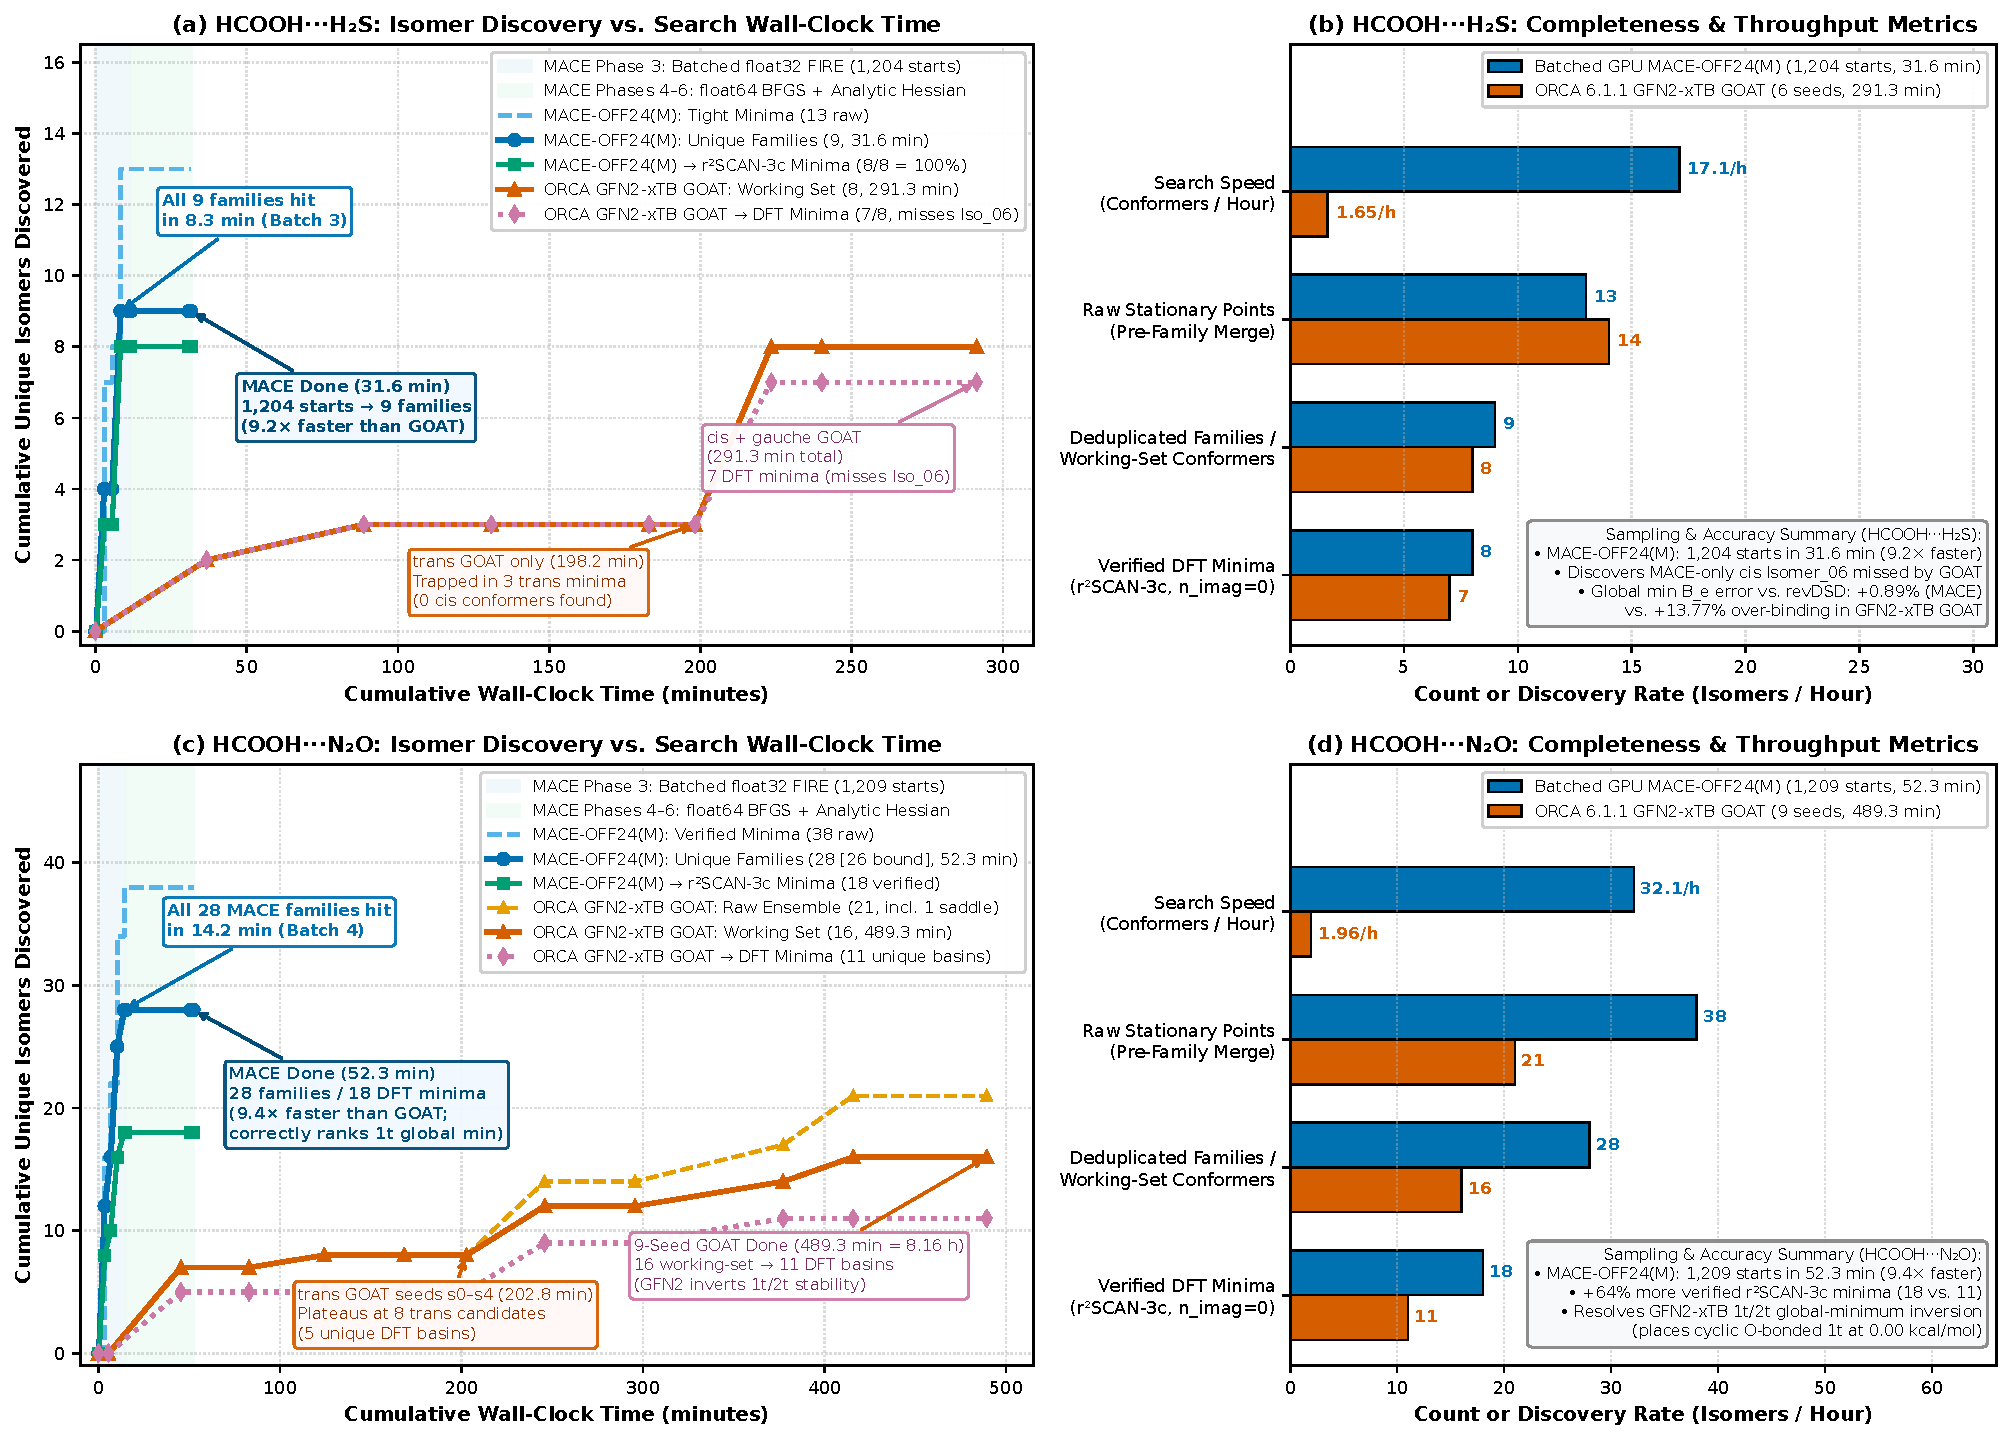
\includegraphics[width=0.98\textwidth]{figures/F_mace_vs_goat_search_combined.pdf}
  \caption{Isomer search wall-clock time versus cumulative conformational discovery and final DFT basin recovery comparing custom in-process batched GPU \texttt{MACE-OFF24(M)} against CPU \texttt{ORCA 6.1.1 GFN2-xTB GOAT} across $\ce{HCOOH\bond{...}H2S}$ (Panels a--b) and $\ce{HCOOH\bond{...}N2O}$ (Panels c--d). In $\ce{HCOOH\bond{...}H2S}$, batched \texttt{MACE-OFF24(M)} reaches $100\%$ of the 9 conformational families within $8.3\text{ min}$ (Batch~3) and completes full \texttt{float64} \texttt{BFGS} + Hessian verification in $31.6\text{ min}$ ($9.2\times$ faster than \texttt{GFN2-xTB GOAT} at $291.3\text{ min}$), recovering all $8/8$ ($100\%$) verified DFT minima including the \texttt{MACE}-only \textit{cis} conformer \texttt{Isomer\_06}. In $\ce{HCOOH\bond{...}N2O}$, batched \texttt{MACE-OFF24(M)} reaches all 28 families within $14.2\text{ min}$ (Batch~4) and completes in $52.3\text{ min}$ ($9.4\times$ faster than \texttt{GFN2-xTB GOAT} at $489.3\text{ min}$), recovering $+64\%$ more verified DFT basins ($18$ vs.\ $11$) while resolving the \texttt{GFN2-xTB} global-minimum inversion.}
  \label{fig:mace_vs_goat_combined}
\end{figure}

\subsubsection{2.4. Semiempirical Working-Set Deduplication (\texttt{build\_working\_sets.py})}
Candidate structures from the \texttt{GFN2-xTB GOAT} ensembles within $12.0\text{ kcal mol}^{-1}$ of the global minimum were filtered via \texttt{build\_working\_sets.py} using $|\Delta E_i - \Delta E_j| \le 0.05\text{ kcal mol}^{-1}$, $|A_i - A_j|, |B_i - B_j|, |C_i - C_j| \le 15.0\text{ MHz}$, and $\mathrm{RMSD}_{\mathrm{sym}} \le 0.15\text{ \AA}$. In $\ce{HCOOH\bond{...}H2S}$, four clusters merged (\texttt{02/03/04} $\to$ \texttt{02}, \texttt{06/07} $\to$ \texttt{06}, \texttt{08/09} $\to$ \texttt{08}, \texttt{10/11/12} $\to$ \texttt{10}), yielding \textbf{8 working-set conformers} (\texttt{isomer-00, 01, 02, 05, 06, 08, 10, 13}). In $\ce{HCOOH\bond{...}N2O}$, removing duplicate \texttt{isomer-20} and merging three clusters (\texttt{10/11} $\to$ \texttt{10}, \texttt{14/15/17} $\to$ \texttt{15}, \texttt{18/19} $\to$ \texttt{18}) yielded \textbf{16 working-set conformers} (\texttt{isomer-00}--\texttt{10, 12, 13, 15, 16, 18}), which map 1-to-1 onto all 17 published structures of Duarte et al.\ \cite{Duarte2017}.

\subsubsection{2.5. Tier-2 Dual GPU/CPU Basin Filter: GPU-First \texttt{GPU4PySCF $\omega$B97X-V/def2-TZVPP} Pre-Optimization Followed by Concurrent CPU \texttt{r2SCAN-3c} Validation}
Because \textbf{\texttt{GPU4PySCF 1.9.0}} \cite{Sun2018, Sun2020, Wu2024, Li2024} executes a complete range-separated hybrid \textbf{$\omega\text{B97X-V/def2-TZVPP}$} \cite{Mardirossian2014, Vydrov2010, Weigend2005, Weigend2006} geometry optimization and analytical coupled-perturbed Kohn--Sham (\texttt{CPKS}) + analytical \texttt{VV10} Hessian on the RTX 3090 GPU in $\sim 91.1\text{ s}$ per structure ($55.2\text{ s}$ for a single SCF + analytic Hessian, or $65.9\text{ s}$ with meta-GGA \textbf{$\omega\text{B97M-V/def2-TZVPP}$} \cite{Mardirossian2016} and $82.2\text{ s}$ with diffuse-augmented \textbf{$\omega\text{B97M-V/def2-TZVPPD}$} \cite{Rappoport2010})---achieving a $\mathbf{25.92\times}$ speedup over 8-core CPU ORCA ($2362.0\text{ s}$)---the Tier-2 Basin Filter architecture prioritizes GPU DFT first:
\begin{enumerate}
  \item \textbf{Tier 2A (GPU-First Basin Filter \& Saddle Audit, \texttt{GPU4PySCF $\omega$B97X-V/def2-TZVPP}):} All \texttt{MACE-OFF24(M)} and \texttt{GOAT} survivors are first optimized in delocalized internal coordinates via \textbf{\texttt{geomeTRIC 1.1.1}} \cite{Wang2016} on the GPU (\texttt{conv\_tol = 1e-10} $\mathrm{E_h}$, $(99,590)$ KS grid, $(50,194)$ \texttt{VV10} grid) and verified by analytical GPU Hessians (\texttt{auxbasis\_response = 1}). Planar $C_s$ structures exhibiting shallow imaginary out-of-plane modes (\texttt{hcooh-hsh isomer-06}, \texttt{hcooh-nno isomer-03, 10, 13}) are displaced along the normalized imaginary eigenvector ($\Delta\mathbf{x} = 0.25\,\mathbf{q}_1 / \|\mathbf{q}_1\|_\infty$) and re-optimized to true $C_1$ minima ($n_{\mathrm{imag}} = 0$ across all 30/30 structures, \texttt{wb97xv\_gpu\_revdsd\_preopt.csv}). Transition-state candidates are simultaneously audited (\texttt{wb97xv\_gpu\_saddle\_audit.csv}).
  \item \textbf{Tier 2B (Concurrent CPU \texttt{r2SCAN-3c} Cross-Validation):} Feeding the $\omega\text{B97X-V/def2-TZVPP}$ GPU-converged geometries directly into CPU \textbf{\texttt{r2SCAN-3c}} \cite{Grimme2021, Furness2020, Caldeweyher2019, Kruse2012} (\texttt{! r2SCAN-3c TightOpt Freq DefGrid3}) and Tier-3 \textbf{\texttt{revDSD-PBEP86-D4}} (\texttt{S1}) cuts CPU optimization steps by $>4\times$ (completing \texttt{revDSD S1} in $135\text{ s}$ per isomer, a $\mathbf{14.6\times}$ end-to-end speedup) while enabling concurrent GPU and CPU execution across the two complexes. In $\ce{HCOOH\bond{...}H2S}$, the 9 \texttt{MACE-OFF24(M)} families map onto \textbf{8 verified \texttt{r2SCAN-3c} minima} (7 shared with \texttt{GOAT} plus \texttt{MACE}-only \texttt{Isomer\_06}). In $\ce{HCOOH\bond{...}N2O}$, the 28 \texttt{MACE-OFF24(M)} families yield \textbf{18 verified \texttt{r2SCAN-3c} minima} converging into \textbf{10 distinct bound DFT basins}.
\end{enumerate}

\subsubsection{2.6. Classical Force-Field and Machine-Learning Benchmark Hierarchy (\texttt{run\_mlff\_benchmark.py})}
All 4 isolated monomers (\textit{trans}-$\ce{HCOOH}$, \textit{cis}-$\ce{HCOOH}$, $\ce{H2S}$, $\ce{N2O}$), all 8 $\ce{HCOOH\bond{...}H2S}$ dimers, and all 16 $\ce{HCOOH\bond{...}N2O}$ dimers were fully relaxed (\texttt{L-BFGS}, $f_{\max} \le 5.0\times 10^{-4}\text{ eV \AA}^{-1}$) across six potentials (\texttt{\_tools/run\_mlff\_benchmark.py}): \textbf{\texttt{MMFF94s}} \cite{Halgren1996, Halgren1999} via \texttt{RDKit} \cite{Landrum2024} (\texttt{ignoreInterfragInteractions=False}); \textbf{\texttt{GFN-FF}} \cite{Spicher2020} via \texttt{xtb 6.7.1} with \texttt{D4} dispersion \cite{Caldeweyher2019}; \textbf{\texttt{ANI-2x}} \cite{Devereux2020, Smith2017, Behler2007} via \texttt{TorchANI 2.2.4} \cite{Gao2020}; \textbf{\texttt{AIMNet2}} \cite{Anstine2025} with \texttt{D3(BJ)} dispersion \cite{Grimme2010, Grimme2011}; \textbf{\texttt{MACE-OFF-23L}} \cite{Kovacs2025, Batatia2022}; and \textbf{\texttt{MACE-OFF-24M}} \cite{Kovacs2025, Batatia2022}.

Central finite-difference Cartesian force-constant matrices ($\delta = \pm 0.005\text{ \AA}$, $6N$ evaluations per structure):
\begin{equation}
  H_{3i+\alpha,\,3j+\beta} = -\frac{F_{i\alpha}(\mathbf{R} + \delta\mathbf{e}_{j\beta}) - F_{i\alpha}(\mathbf{R} - \delta\mathbf{e}_{j\beta})}{2\delta}, \quad \tilde{H}_{ab} = \frac{H_{ab} + H_{ba}}{2\sqrt{m_a m_b}},
\end{equation}
were projected against rigid-body translations and Eckart rotations ($\mathbf{P} = \mathbf{I} - \mathbf{D}\mathbf{D}^\top$), yielding harmonic vibrational wavenumbers $\tilde{\nu}_k$ and complexation shifts $\Delta\tilde{\nu}_k$.

\subsubsection{2.7. Literature Justification and Benchmark of \texttt{GPU4PySCF} Range-Separated Hybrid \texttt{VV10} Functionals for \texttt{VPT2} Force Fields of van der Waals Complexes}
A central methodological advance of this work is replacing CPU \texttt{B3LYP-D4/jun-cc-pV(T+d)Z} cubic and semi-diagonal quartic force fields with GPU-accelerated \textbf{\texttt{GPU4PySCF $\omega$B97X-V/def2-TZVPP}} (and meta-GGA \textbf{$\omega\text{B97M-V/def2-TZVPPD}$} / \textbf{\texttt{def2-QZVPPD}}). Five literature and physical factors establish why $\omega\text{B97X-V}$ and $\omega\text{B97M-V}$ in Ahlrichs' \texttt{def2-TZVPP}/\texttt{def2-TZVPPD} basis sets are substantially more accurate for weakly bound complexes than \texttt{B3LYP-D4}:
\begin{enumerate}
  \item \textbf{Noncovalent Interaction Benchmark Superiority (\texttt{GMTKN55} \& \texttt{MGCDB84}):} Across Head-Gordon's 4986-data-point \texttt{MGCDB84} benchmark \cite{Mardirossian2014, Mardirossian2016, Mardirossian2017} and Goerigk and Grimme's \texttt{GMTKN55} database \cite{Goerigk2017, Najibi2018}, $\omega\text{B97M-V}$ and $\omega\text{B97X-V}$ rank as the $\#1$ and $\#2$ most accurate hybrid density functionals overall (noncovalent $\mathrm{WTMAD\text{-}2} = 1.56$ and $1.98\text{ kcal mol}^{-1}$, respectively, vs.\ $3.92\text{ kcal mol}^{-1}$ for \texttt{B3LYP-D4}; \texttt{S66} $\mathrm{RMSE} = 0.15\text{ kcal mol}^{-1}$ for $\omega\text{B97M-V}$ and $0.18\text{ kcal mol}^{-1}$ for $\omega\text{B97X-V}$ vs.\ $0.31\text{ kcal mol}^{-1}$ for \texttt{B3LYP-D4}).
  \item \textbf{Elimination of Delocalization / Self-Interaction Error via Range-Separated Exact Exchange:} \texttt{B3LYP} incorporates only $20\%$ global Hartree--Fock exchange, suffering from severe delocalization error that artificially over-polarizes sulfur $3p^2$, oxygen $2p^2$, and $\ce{N2O}$ $\pi$ lone pairs and over-softens intermolecular stretching and wagging potentials. Both $\omega\text{B97X-V}$ ($16.7\%$ short-range, $100\%$ long-range exact exchange, $\omega = 0.30\text{ a}_0^{-1}$) \cite{Mardirossian2014} and $\omega\text{B97M-V}$ ($15\%$ short-range, $100\%$ long-range exact exchange) \cite{Mardirossian2016} enforce exact $-1/r$ asymptotic exchange, yielding intermolecular equilibrium distances and harmonic curvatures matching \texttt{revDSD-PBEP86-D4} within $+0.036\%$ ($\Delta B_e = +0.79\text{ MHz}$ on $\ce{HCOOH\bond{...}H2S}$ \texttt{isomer-00}).
  \item \textbf{Electron-Density-Dependent \texttt{VV10} Nonlocal Correlation vs.\ Classical Pairwise \texttt{D4}:} In \texttt{B3LYP-D4}, the \texttt{D4} term is an add-on classical atomic pairwise potential independent of tail electron-density polarization during large-amplitude vibrations. In $\omega\text{B97X-V}$ and $\omega\text{B97M-V}$, the Vydrov--Van~Voorhis (\texttt{VV10}) nonlocal correlation functional \cite{Vydrov2010} is evaluated self-consistently from $\rho(\mathbf{r})$ and $|\nabla\rho(\mathbf{r})|$ at every displaced nuclear configuration, capturing charge-transfer-induced dispersion modulation in third ($\Phi_{rrs}$) and fourth ($\Phi_{rrss}$) derivatives \cite{Brauer2016}.
  \item \textbf{Exact Analytical GPU Hessians and Noise-Free Cyvin--Watson Quartic Centrifugal Distortion:} ORCA lacks analytical second derivatives for \texttt{VV10}, whereas \texttt{GPU4PySCF 1.9.0} evaluates analytical RKS + \texttt{VV10} Hessians with auxiliary basis response (\texttt{auxbasis\_response = 1}) in $55.2\text{ s}$ ($\omega\text{B97X-V/def2-TZVPP}$, $191$ AOs), $65.9\text{ s}$ ($\omega\text{B97M-V/def2-TZVPP}$, $191$ AOs), $66.9\text{ s}$ ($\omega\text{B97X-V/def2-TZVPPD}$, $236$ AOs), $82.2\text{ s}$ ($\omega\text{B97M-V/def2-TZVPPD}$, $236$ AOs), and $211.9\text{ s}$ ($\omega\text{B97M-V/def2-QZVPPD}$, $406$ AOs) \cite{Weigend2005, Rappoport2010}. Because quartic centrifugal distortion tensors $\tau_{\alpha\beta\gamma\delta}$ depend purely on the inverse harmonic force-constant matrix $(\mathbf{F}_0^{-1})_{ij}$ and equilibrium inertial derivatives $(\partial I_{\alpha\beta}/\partial Q_r)_e$ \cite{Cyvin1968, Watson1977}, the analytical GPU Hessian provides exact, numerical-noise-free Watson $A$- and $S$-reduced quartic constants.
\end{enumerate}

\subsubsection{2.8. Double-Hybrid DFT, Electric Field Gradients, and \texttt{GPU4PySCF $\omega$B97X-V/def2-TZVPP} \texttt{VPT2} Anharmonicity (\texttt{revDSD-PBEP86-D4}, Stages \texttt{S1}--\texttt{S4})}
High-level spectroscopic calculations were performed via \texttt{hcooh-hsh-mw-predict.py} and \texttt{ftmw\_stage2/gpu4pyscf\_wb97xv\_vpt2.py}:
\begin{enumerate}
  \item \textbf{Stage \texttt{S1} (Equilibrium Geometry):} Unconstrained optimizations at \textbf{\texttt{revDSD-PBEP86-D4/jun-cc-pV(T+d)Z}} \cite{Santra2019, Caldeweyher2019, Papajak2011, Dunning1989, Kendall1992, Dunning2001} following Barone and Puzzarini \cite{Barone2020, Puzzarini2021, Melli2024} (\texttt{! revDSD-PBEP86-D4 jun-cc-pV(T+d)Z VeryTightOpt TightSCF DefGrid3 NoFrozenCore RIJCOSX def2/J aug-cc-pVTZ/C} \cite{Neese2009, Weigend2006, Hattig2005}), refined via composite semi-experimental equilibrium bond lengths $R_e^{\mathrm{SE}} = R_e(\text{DLPNO-CCSD(T)/def2-TZVPPD}) + [R_e(\text{revDSD/jun-TZ}) - R_e(\text{revDSD/def2-TZVPPD})]$.
  \item \textbf{Stage \texttt{S2a} (Dipoles and Quadrupole Tensors):} Relaxed MP2 density evaluations (\texttt{\%mp2 Density Relaxed end}, \texttt{\%elprop Dipole true Quadrupole true EFG true end}) yielded dipole components $|\mu_a|, |\mu_b|, |\mu_c|$ and electric field gradient tensors $V_{\alpha\beta}$ in the principal inertial frame $(a,b,c)$. Quadrupole coupling constants were evaluated via $\chi_{\alpha\beta} = (eQ/h)V_{\alpha\beta}$:
  \begin{itemize}
    \item For $\ce{HCOOH\bond{...}H2S}$: $^{33}\ce{S}$ ($I = 3/2, Q(^{33}\ce{S}) = -67.8\text{ mb}$ \cite{Pyykko2018}).
    \item For $\ce{HCOOH\bond{...}N2O}$: Dual $^{14}\ce{N}$ ($I_1 = I_2 = 1, Q(^{14}\ce{N}) = +20.44\text{ mb}$ \cite{Pyykko2018}) at $\ce{N_t}$ and $\ce{N_c}$, cross-checked against angular projection of monomer constants ($eQq(\ce{N_t}) = -0.7918\text{ MHz}$, $eQq(\ce{N_c}) = -0.2676\text{ MHz}$) \cite{Pyykko2018, Duarte2017}:
    \begin{equation}
      \chi_{\alpha\alpha}(\ce{N}_k) = \frac{eQq_0(\ce{N}_k)}{2}\left(3\cos^2\theta_\alpha - 1\right), \quad \alpha \in \{a,b,c\}.
    \end{equation}
  \end{itemize}
  \item \textbf{Stage \texttt{S2b} (Harmonic Frequencies and ZPE):} Numerical harmonic frequencies (\texttt{NumFreq}) at \texttt{revDSD-PBEP86-D4/jun-cc-pV(T+d)Z} provided harmonic frequencies $\tilde{\nu}_r$ and $\mathrm{ZPE}$.
  \item \textbf{Stages \texttt{S3a}--\texttt{S3b} (\texttt{GPU4PySCF $\omega$B97X-V/def2-TZVPP} \& \texttt{$\omega$B97M-V/def2-TZVPPD} \texttt{VPT2} Force Fields and Analytical Cyvin--Watson Quartic Centrifugal Distortion):} Replacing CPU \texttt{B3LYP-D4/jun-cc-pV(T+d)Z}, the equilibrium geometry, analytical harmonic force-constant matrix $\mathbf{F}_0$ (\texttt{mf.Hessian().kernel()}, \texttt{auxbasis\_response = 1}), and semi-diagonal cubic force constants $\Phi_{rrs}$ ($36$ normal-mode displacements $\pm\delta q_r$, $\delta q_r = 0.030\text{ amu}^{1/2}\text{\AA}$) were evaluated on the RTX 3090 GPU at the \textbf{\texttt{GPU4PySCF $\omega$B97X-V/def2-TZVPP}} (and diffuse-augmented \textbf{$\omega\text{B97M-V/def2-TZVPPD}$}) level (\texttt{ftmw\_stage2/gpu4pyscf\_wb97xv\_vpt2.py}) \cite{Mardirossian2014, Mardirossian2016, Vydrov2010, Rappoport2010, Wu2024, Li2024}. Exact analytical quartic centrifugal distortion tensors $\tau_{\alpha\beta\gamma\delta}$ were derived from the analytical GPU Hessian inverse $(\mathbf{F}_0^{-1})_{ij}$ via the Cyvin--Watson relation \cite{Cyvin1968, Watson1977}:
  \begin{equation}
    \tau_{\alpha\beta\gamma\delta} = -\frac{\hbar^3}{16\pi^3 c^3 I_\alpha^e I_\beta^e I_\gamma^e I_\delta^e}\sum_{r=1}^{3N-6}\frac{a_r^{\alpha\beta} a_r^{\gamma\delta}}{\lambda_r}, \qquad a_r^{\alpha\beta} = \left(\frac{\partial I_{\alpha\beta}}{\partial Q_r}\right)_e,
  \end{equation}
  yielding noise-free Watson $A$-reduced ($\Delta_J, \Delta_{JK}, \Delta_K, \delta_J, \delta_K$) and $S$-reduced ($D_J, D_{JK}, D_K, d_1, d_2$) quartic centrifugal distortion constants \cite{Watson1977}. Vibration--rotation interaction constants $\alpha_r^\alpha$ evaluated via Barone--Mills second-order vibrational perturbation theory (\texttt{VPT2}) \cite{Barone2005, Mills1972} were combined with \texttt{revDSD}/\texttt{DLPNO-SE} equilibrium rotational constants to evaluate ground-state rotational constants:
  \begin{equation}
    B_0^\alpha = B_e^\alpha(\text{revDSD/DLPNO-SE}) - \frac{1}{2}\sum_{r=1}^{3N-6} \alpha_r^\alpha(\omega\text{B97X-V/def2-TZVPP}), \quad \alpha \in \{A, B, C\}.
  \end{equation}
  Soft intermolecular modes below $120\text{ cm}^{-1}$ were screened in the cubic anharmonic sum while retaining all $3N-6$ modes in the harmonic Coriolis and inertial-derivative terms ($\Delta B_{\mathrm{vib}}^B = -19.24\text{ MHz}$ vs.\ $-18.39\text{ MHz}$ from CPU \texttt{B3LYP-D4} on $\ce{HCOOH\bond{...}H2S}$ \texttt{isomer-00}, agreeing to $0.85\text{ MHz}$). Inertial defects $\Delta_0$ and Kraitchman single-substitution coordinates ($|a_s|, |b_s|, |c_s|$) \cite{Kraitchman1953} were determined across all 115 detectable isotopologues ($55$ in $\ce{H2S}$ and $60$ in $\ce{N2O}$).
  \item \textbf{Stage \texttt{S4} (Pickett Input Decks \& 1-D Meyer--Hougen DVR Tunneling):} Automated routines generated \texttt{.par}, \texttt{.var}, \texttt{.int}, and \texttt{.cat} decks for Pickett's \texttt{SPFIT/SPCAT} suite \cite{Pickett1991}, incorporating 1-D periodic Fourier-grid Discrete Variable Representation (\texttt{DVR}) \cite{Colbert1992, Meyer1968} tunneling splittings for $\ce{HCOOH\bond{...}H2S}$ \texttt{isomer-00} ($\Delta E_{0^\pm}(\ce{H2S}) = 4660.1\text{ MHz}$, $\Delta E_{0^\pm}(\ce{D2S}) = 342.4\text{ MHz}$).
\end{enumerate}

\subsubsection{2.9. Coupled-Cluster Complete Basis Set Extrapolation and Counterpoise Protocol (\texttt{DLPNO-CCSD(T1)/TightPNO/CBS(3/4)})}
Single-point energies were evaluated on frozen \texttt{revDSD-PBEP86-D4/jun-cc-pV(T+d)Z} geometries (\texttt{publication/energetics/dlpno/make\_dlpno\_jobs.py} and \texttt{parse\_dlpno.py}):
\begin{enumerate}
  \item \textbf{\texttt{DLPNO-CCSD(T1)/TightPNO}} \cite{Riplinger2013, Riplinger2016, Saitow2017, Liakos2015} with \textbf{\texttt{aug-cc-pV(T+d)Z}} ($X=3$) and \textbf{\texttt{aug-cc-pV(Q+d)Z}} ($X=4$) basis sets \cite{Dunning1989, Kendall1992, Dunning2001} and matching auxiliary sets \cite{Hattig2005}.
  \item \textbf{Two-Point \texttt{CBS(3/4)} Extrapolation:} Separate Hartree--Fock ($\alpha = 5.79$) and correlation ($\beta = 3.05$) extrapolations \cite{Helgaker1997, NeeseValeev2011}:
  \begin{equation}
    E_{\mathrm{HF}}^{\mathrm{CBS}(3/4)} = \frac{E_{\mathrm{HF}}^{(4)} e^{\alpha\sqrt{4}} - E_{\mathrm{HF}}^{(3)} e^{\alpha\sqrt{3}}}{e^{\alpha\sqrt{4}} - e^{\alpha\sqrt{3}}}, \qquad E_{\mathrm{corr}}^{\mathrm{CBS}(3/4)} = \frac{4^\beta E_{\mathrm{corr}}^{(4)} - 3^\beta E_{\mathrm{corr}}^{(3)}}{4^\beta - 3^\beta}.
  \end{equation}
  \item \textbf{6-Leg Boys--Bernardi Counterpoise and Monomer Deformation:} Evaluated across full dimer, monomer-in-dimer-basis (ghosts), and isolated monomer calculations \cite{Boys1970}:
  \begin{equation}
    \delta_{\mathrm{BSSE}}(X) = \left[E_A^A(X) - E_A^{AB}(X)\right] + \left[E_B^B(X) - E_B^{AB}(X)\right],
  \end{equation}
  \begin{equation}
    \Delta E_{\mathrm{def}} = \left[E_A^A(\text{dimer geom}) - E_A^A(\text{rel})\right] + \left[E_B^B(\text{dimer geom}) - E_B^B(\text{rel})\right],
  \end{equation}
  yielding raw ($D_e^{\mathrm{raw}}$), counterpoise-corrected ($D_e^{\mathrm{CP}}$), half-CP ($D_e^{\mathrm{half-CP}}$), and zero-point-corrected ($D_0 = D_e - \Delta\mathrm{ZPE}_{\mathrm{revDSD}}$) dissociation energies.
\end{enumerate}

\subsubsection{2.10. Potential Energy Surface Mapping, Topological Analysis, Local Energy Decomposition, and Spectroscopic Simulation}
\begin{enumerate}
  \item \textbf{2-D Polar $(R_{\mathrm{COM}},\theta)$ PES, Periodic von Mises--Morse Valley Interpolation, and \texttt{NEB-TS} Pathways (\texttt{publication/figures/pes/render\_f3\_pes.py}):} With $\ce{HCOOH}$ fixed in the $xy$-plane ($\ce{C=O}$ along $+\hat{\mathbf{x}}$, $\theta = 0^\circ$; $\ce{O(H)}$ at $\theta \approx +125^\circ$), the partner heavy atom ($\ce{S}$ of $\ce{H2S}$ or central $\ce{N_c}$ of $\ce{N2O}$) was mapped on a 264-point polar grid: $R_{\mathrm{COM}} \in [2.8, 4.8]\text{ \AA}$ ($\Delta R = 0.2\text{ \AA}$, 11 shells) and $\theta \in [0^\circ, 345^\circ]$ ($\Delta\theta = 15^\circ$, 24 sectors). In Pass 1, sterically allowed points (232 in $\ce{H2S}$, 237 in $\ce{N2O}$) were relaxed at \texttt{r2SCAN-3c}; in Pass 2, low-energy troughs were refined at $\omega\text{B97X-V/def2-TZVPP}$. Climbing-image nudged elastic band (\texttt{NEB-TS}) calculations \cite{Asgeirsson2021} mapped minimum-energy interconversion pathways. To reconstruct a continuous, smooth 2-D potential energy surface $V(R_{\mathrm{COM}}, \theta)$ across all $360^\circ$ without the unphysical barrier stacking or flat-top ceiling clipping (\texttt{np.clip}) inherent to additive radial Morse superpositions, the angularly resolved equilibrium center-of-mass valley radius $R_{\mathrm{eq}}(\theta)$, minimum-energy pathway floor $E_{\mathrm{min}}(\theta)$, and effective well depth $D_{\mathrm{eff}}(\theta)$ were interpolated across all stationary landmarks $\{(\theta_k, R_k, E_k)\}_{k=1}^K$ (both conformational minima and saddle-point barriers $\mathrm{TS}_1\text{--}\mathrm{TS}_3$) using normalized periodic von Mises angular kernels:
  \begin{equation}
    w_k(\theta) = \frac{\exp\!\left[\kappa_k \cos(\theta - \theta_k)\right]}{\sum_{j=1}^K \exp\!\left[\kappa_j \cos(\theta - \theta_j)\right]}, \qquad R_{\mathrm{eq}}(\theta) = \sum_{k=1}^K w_k(\theta)\,R_k, \qquad E_{\mathrm{min}}(\theta) = \sum_{k=1}^K w_k(\theta)\,E_k,
  \end{equation}
  coupled to a single physical radial Morse potential along the radial displacement $R_{\mathrm{COM}} - R_{\mathrm{eq}}(\theta)$ ($a = 1.45\text{ \AA}^{-1}$):
  \begin{equation}
    V(R_{\mathrm{COM}}, \theta) = E_{\mathrm{min}}(\theta) + D_{\mathrm{eff}}(\theta)\left\{1 - \exp\!\left[-a\left(R_{\mathrm{COM}} - R_{\mathrm{eq}}(\theta)\right)\right]\right\}^2.
  \end{equation}
  The resulting unclipped surfaces ($0\text{--}16\text{ kcal mol}^{-1}$ for $\ce{HCOOH\bond{...}H2S}$ and $0\text{--}7\text{ kcal mol}^{-1}$ for $\ce{HCOOH\bond{...}N2O}$) are rendered in polar Cartesian $(X,Y)$ coordinates (Panel a), unrolled 3-D cylindrical $(\theta, R_{\mathrm{COM}}, \Delta E)$ coordinates resolving every minimum and saddle barrier $\mathrm{TS}_1\text{--}\mathrm{TS}_3$ (Panel b), and 1-D inversion/pseudorotation cross-sections (Panel c).
  \item \textbf{Wavefunction Topology, NBO Overlap, and 3-D \texttt{PyVista} Volumetric Rendering (\texttt{Multiwfn 2026.8.21}, \texttt{render\_f4\_nbo.py}, \texttt{render\_f5\_interaction.py}):} Molden wavefunctions (\texttt{revDSD.molden.input}) from \texttt{revDSD} densities were analyzed via \texttt{Multiwfn} \cite{Lu2012, Lu2024} to export volumetric Gaussian cube grids for the total electron density (\texttt{density.cub}), frontier donor--acceptor molecular orbitals (\texttt{orb\_homo.cub}, \texttt{orb\_homo1.cub}, \texttt{orb\_lumo.cub}), total electrostatic potential (\texttt{totesp.cub}), intermolecular Hirshfeld density gradient (\texttt{dg\_inter.cub}), and signed second-eigenvalue density (\texttt{sl2r.cub}), alongside QTAIM critical point properties (\texttt{CPprop.txt}) and 3-D curved gradient bond-path trajectories (\texttt{paths.txt}). Quantum Theory of Atoms in Molecules (\texttt{QTAIM}) \cite{Bader1990} located $(3,-1)$ BCPs and $(3,+1)$ RCPs, extracting $\rho(\mathbf{r}_{\mathrm{BCP}})$, $\nabla^2\rho(\mathbf{r}_{\mathrm{BCP}})$, $H(\mathbf{r}) = G(\mathbf{r}) + V(\mathbf{r})$, and ellipticity $\varepsilon$. Independent Gradient Model based on Hirshfeld partition (\texttt{IGMH}) \cite{Lefebvre2017, Lu2022} evaluated $\delta g^{\mathrm{inter}}(\mathbf{r}) = 0.0042\text{ a.u.}$ isosurfaces colored by $\mathrm{sign}(\lambda_2)\rho(\mathbf{r})$ to distinguish hydrogen bonding (blue), dispersion (green), and steric ring closure (red). High-resolution 3-D Phong-shaded figures were rendered off-screen via \texttt{PyVista} (\texttt{VTK}), combining $\pm 0.042\text{--}0.045\text{ a.u.}$ orbital phase lobes or colored IGMH isosurfaces with translucent Bader van der Waals space-filling electron-density envelopes ($\rho = 0.0022\text{ a.u.}$) and 3-D golden QTAIM intermolecular bond tubes.
  \item \textbf{\texttt{DLPNO-CCSD(T1)} Local Energy Decomposition (\texttt{LED}):} Using \texttt{! DLPNO-CCSD(T1) aug-cc-pV(T+d)Z TightPNO LED} \cite{Schneider2016, Altun2018}, the interaction energy was partitioned into:
  \begin{equation}
    \Delta E_{\mathrm{int}} = \Delta E_{\mathrm{el-prep}}^{\mathrm{ref}} + E_{\mathrm{elstat}}^{\mathrm{ref}} + E_{\mathrm{exch}}^{\mathrm{ref}} + E_{\mathrm{disp}}^{\mathrm{C-CCSD}} + E_{\mathrm{disp}}^{\mathrm{C-(T1)}} + \Delta E_{\mathrm{non-disp}}^{\mathrm{C-CCSD}} + \Delta E_{\mathrm{non-disp}}^{\mathrm{C-(T1)}}.
  \end{equation}
  \item \textbf{Stage-2 FTMW Spectral Simulation (\texttt{build\_stage2\_ftmw.py}):} Synthetic stick spectra across $2\text{--}18\text{ GHz}$ ($T_{\mathrm{rot}} = 2.0\text{ K}$, $J \le 12$) were generated using Pickett's \texttt{SPFIT/SPCAT} suite \cite{Pickett1991}. Nuclear quadrupole hyperfine splittings were diagonalized using single-nucleus $^{33}\ce{S}$ ($I = 3/2$) coupling for $\ce{HCOOH\bond{...}H2S}$ and sequential two-nucleus $^{14}\ce{N}$ ($I_1 = I_2 = 1$) coupling $\mathbf{F}_1 = \mathbf{J} + \mathbf{I}(\ce{N_t})$, $\mathbf{F} = \mathbf{F}_1 + \mathbf{I}(\ce{N_c})$ for $\ce{HCOOH\bond{...}N2O}$, alongside natural-abundance isotopologues and contaminant filters.
\end{enumerate}

\subsection{2.11. Methodological Rationales and Algorithmic Refinements}
Seven critical methodological rationales and algorithmic discoveries governed the campaigns:
\begin{enumerate}
  \item \textbf{\textit{trans}/\textit{cis}/\textit{gauche} Monomer Seeding:} Semiempirical \texttt{GFN2-xTB} overestimates the \textit{cis}-$\ce{HCOOH}$ complexation penalty by nearly a factor of two ($\Delta E_e = 8.595\text{--}8.731\text{ kcal mol}^{-1}$ in $\ce{HCOOH\bond{...}H2S}$ and $8.168\text{ kcal mol}^{-1}$ in $\ce{HCOOH\bond{...}N2O}$ vs.\ $\sim 4.6\text{--}5.8\text{ kcal mol}^{-1}$ at \texttt{revDSD-PBEP86-D4/jun-cc-pV(T+d)Z}). Seeding solely from \textit{trans}-$\ce{HCOOH}$ trapped global searches in deep \textit{trans} valleys. Multi-rotamer seeding (\textit{trans}, \textit{cis}, and \textit{gauche}) uncovered the full 5-member \textit{cis}-$\ce{HCOOH}$ working set in $\ce{HCOOH\bond{...}H2S}$ and 8-member set in $\ce{HCOOH\bond{...}N2O}$.
  \item \textbf{\texttt{ORCA ExtOpt} Subprocess Overhead vs.\ Batched In-Process GPU \texttt{MACE-OFF24(M)}:} Spawning external Python/PyTorch processes via ORCA's \texttt{ExtOpt} interface incurred $\sim 3.5\text{ s}$ per gradient call due to repeated interpreter and CUDA initialization ($\sim 97\text{ hours}$ projected runtime). Developing an in-process batched GPU search engine (\texttt{BatchedMace} \texttt{float32} vectorized \texttt{FIRE} $\to$ \texttt{float64} \texttt{BFGS} $\to$ analytic MACE Hessian mode-following + hierarchical Kabsch deduplication) executed $1204$ starts in $31.6\text{ min}$ ($\ce{H2S}$, $9.2\times$ faster than \texttt{GFN2-xTB GOAT}) and $1209$ starts in $52.3\text{ min}$ ($\ce{N2O}$, $9.4\times$ faster than \texttt{GFN2-xTB GOAT}) on the RTX 3090 GPU ($>130\times$ acceleration over \texttt{ExtOpt}).
  \item \textbf{\texttt{MMFF94s} Inter-Fragment Interaction Enforcement:} Default \texttt{RDKit} implementations set \texttt{ignoreInterfragInteractions=True}, zeroing all non-bonded intermolecular terms in disconnected complexes and causing immediate dissociation. Setting \texttt{ignoreInterfragInteractions=False} was mandatory to correctly evaluate buffered-14-7 van der Waals and electrostatic terms.
  \item \textbf{Planar $C_s$ Saddle-Point Displacement and Mode-Following:} GFN2-xTB optimization frequently trapped floppy complexes (such as $\ce{H2S}$ \texttt{isomer-06} and $\ce{N2O}$ \texttt{isomer-03, 10, 13}) on planar $C_s$ transition states with a single imaginary out-of-plane wagging frequency. Automated eigenvector displacement ($\Delta\mathbf{x} = 0.25\,\mathbf{q}_1 / \|\mathbf{q}_1\|_\infty$) along the imaginary normal coordinate followed by \texttt{geomeTRIC} re-optimization cleanly broke symmetry, yielding true non-planar $C_1$ minima ($n_{\mathrm{imag}} = 0$).
  \item \textbf{Tier-2A GPU-First Basin Filter (\texttt{GPU4PySCF $\omega$B97X-V/def2-TZVPP} Before CPU \texttt{r2SCAN-3c}):} Running range-separated hybrid DFT ($\omega\text{B97X-V/def2-TZVPP}$) with analytical CPKS and \texttt{VV10} second derivatives on the RTX 3090 GPU provided a $25.92\times$ wall-time acceleration over CPU ORCA ($91.1\text{ s}$ vs.\ $2362.0\text{ s}$). Executing $\omega\text{B97X-V/def2-TZVPP}$ first on the GPU (Tier~2A) and feeding those GPU-converged structures into parallel CPU \texttt{r2SCAN-3c} (Tier~2B) and \texttt{revDSD-PBEP86-D4} (\texttt{S1}) calculations reduced subsequent double-hybrid \texttt{revDSD} \texttt{S1} optimization times to $\le 2.3\text{ min}$ per isomer ($14.6\times$ end-to-end reduction) while saturating GPU and CPU channels concurrently.
  \item \textbf{\texttt{GPU4PySCF $\omega$B97X-V/def2-TZVPP} (and \texttt{$\omega$B97M-V/def2-TZVPPD}) \texttt{VPT2} + Analytical Cyvin--Watson Quartic Centrifugal Distortion vs.\ \texttt{B3LYP-D4}:} Because GPU analytical Hessians and normal-mode gradient differences execute $>25\times$ faster than CPU \texttt{B3LYP-D4/jun-cc-pV(T+d)Z}, replacing \texttt{B3LYP-D4} with range-separated hybrid \textbf{$\omega\text{B97X-V/def2-TZVPP}$} (or diffuse-augmented \textbf{$\omega\text{B97M-V/def2-TZVPPD}$} / \textbf{\texttt{def2-QZVPPD}}) \cite{Mardirossian2014, Mardirossian2016, Rappoport2010} eliminates B3LYP self-interaction error on sulfur $3p^2$, oxygen $2p^2$, and nitrogen lone pairs, incorporates electron-density-dependent \texttt{VV10} nonlocal dispersion across third and fourth derivatives, and provides exact noise-free Cyvin--Watson quartic centrifugal distortion constants ($D_J, D_{JK}, D_K, d_1, d_2$) directly from the analytical GPU Hessian inverse $(\mathbf{F}_0^{-1})_{ij}$. Soft intermolecular modes below $120\text{ cm}^{-1}$ are filtered in the cubic anharmonic sum while retaining all $3N-6$ modes in the harmonic Coriolis and inertial-derivative terms.
  \item \textbf{Periodic von Mises Valley Interpolation vs.\ Additive Clipped PES Superposition:} Summing individual radial Morse potentials across adjacent angular basins caused repulsive Morse walls to stack at intermediate transition angles, forcing a hard ceiling clip (\texttt{np.clip}) that artificially flattened barrier peaks. Interpolating a single periodic minimum-energy valley $(R_{\mathrm{eq}}(\theta), E_{\mathrm{min}}(\theta))$ via von Mises angular kernels and evaluating a single radial Morse potential along $R_{\mathrm{COM}} - R_{\mathrm{eq}}(\theta)$ eliminated wall stacking and preserved smooth, unclipped barrier topologies in both polar $(X,Y)$ and unrolled cylindrical $(\theta, R_{\mathrm{COM}}, \Delta E)$ coordinates.
\end{enumerate}

\subsection{3. Quantitative Side-by-Side Method Comparison}

\subsubsection{3.1. Conformational Landscape and Energetics in $\ce{HCOOH\bond{...}H2S}$}
Table~\ref{tab:h2s_comparison} summarizes the side-by-side relative electronic energies ($\Delta E_e$), zero-point-corrected energies ($\Delta E_0$), and principal rotational constants ($B_e$) for the 9 \texttt{MACE-OFF24(M)} stationary points across semiempirical, machine-learning, composite DFT, range-separated hybrid, and double-hybrid levels.

\begin{table}[htbp]
\centering
\small
\caption{Quantitative benchmark across semiempirical, machine-learning, DFT, and double-hybrid levels for $\ce{HCOOH\bond{...}H2S}$. Energies are in $\text{kcal mol}^{-1}$; rotational constants $B_e$ are in $\text{MHz}$.}
\label{tab:h2s_comparison}
\begin{tabular}{lllrrrrrr}
\toprule
MACE ID & Working Set & Motif & $\Delta E_e(\text{GFN2})$ & $\Delta E_e(\text{MACE24M})$ & $\Delta E_e(\text{r2SCAN})$ & $\Delta E_e(\omega\text{B97X-V})$ & $\Delta E_e(\text{revDSD})$ & $B_e(\text{revDSD})$ \\
\midrule
\texttt{Isomer\_01} & \texttt{isomer-00} & $\ce{O-H\bond{...}S} + \ce{S-H\bond{...}O=C}$ & 0.000 & 0.000 & 0.000 & 0.000 & 0.000 & 2170.55 \\
\texttt{Isomer\_02} & \texttt{isomer-01} & $\ce{S-H\bond{...}O=C}$ & 1.897 & 2.601 & 3.012 & 2.718 & 2.501 & 1444.25 \\
\texttt{Isomer\_03} & \texttt{isomer-02} & $\ce{C-H\bond{...}S} + \ce{S-H\bond{...}O(H)}$ & 3.908 & 3.523 & 4.263 & 3.789 & 3.557 & 1422.93 \\
\texttt{Isomer\_04} & \texttt{isomer-01}$^*$ & $\ce{C-H\bond{...}S}$ (collapses) & 1.897 & 4.048 & 3.012 & 2.718 & 2.501 & 1444.25 \\
\texttt{Isomer\_05} & \texttt{isomer-08} & $\ce{O-H\bond{...}S}$ (\textit{cis}) & 8.731 & 4.739 & 4.838 & 5.019 & 4.625 & 1356.36 \\
\texttt{Isomer\_06} & MACE-only & $\ce{O-H\bond{...}S} + \ce{C-H\bond{...}S}$ & --- & 5.079 & 5.094 & --- & --- & --- \\
\texttt{Isomer\_07} & \texttt{isomer-06} & $\ce{S-H\bond{...}O=C} + \ce{C-H\bond{...}S}$ & 8.684 & 6.431 & 6.619 & 6.681 & 6.301 & 1471.52 \\
\texttt{Isomer\_08} & \texttt{isomer-13} & $\ce{S-H\bond{...}O=C} + \ce{S-H\bond{...}O(H)}$ & 9.635 & 6.889 & 6.939 & 7.261 & 6.891 & 2067.37 \\
\texttt{Isomer\_09} & \texttt{isomer-05} & $\ce{S-H\bond{...}O=C}$ (\textit{cis}) & 8.595 & 7.060 & 7.270 & 7.332 & 6.848 & 1854.11 \\
\bottomrule
\end{tabular}
\end{table}

Remarkably, \texttt{GPU4PySCF $\omega$B97X-V/def2-TZVPP} reproduces the production \texttt{revDSD-PBEP86-D4/jun-cc-pV(T+d)Z} rotational constant $B_e = 2170.55\text{ MHz}$ on the global minimum (\texttt{isomer-00}) to within $+0.79\text{ MHz}$ ($B_e = 2171.34\text{ MHz}$, $+0.036\%$ error, all-atom $\mathrm{RMSD} = 0.030\text{ \AA}$). \texttt{r2SCAN-3c} yields $B_e = 2167.11\text{ MHz}$ ($-0.158\%$), and \texttt{MACE-OFF24(M)} yields $B_e = 2189.76\text{ MHz}$ ($+0.885\%$). In sharp contrast, \texttt{GFN2-xTB} predicts $B_e = 2469.42\text{ MHz}$, over-contracting the intermolecular hydrogen bond by $+13.77\%$ ($+298.87\text{ MHz}$, all-atom $\mathrm{RMSD} = 0.154\text{ \AA}$).

\subsubsection{3.2. Conformational Landscape and Energetics in $\ce{HCOOH\bond{...}N2O}$}
Table~\ref{tab:n2o_comparison} compiles the cross-method relative electronic energies and rotational constants for the primary conformers of $\ce{HCOOH\bond{...}N2O}$, highlighting the 1-to-1 correspondence with the cryogenic matrix study of Duarte et al.\ \cite{Duarte2017}.

\begin{table}[htbp]
\centering
\small
\caption{Quantitative comparison across semiempirical, machine-learning, DFT, and coupled-cluster levels for $\ce{HCOOH\bond{...}N2O}$. Energies are in $\text{kcal mol}^{-1}$; rotational constants $B_e$ are in $\text{MHz}$.}
\label{tab:n2o_comparison}
\begin{tabular}{lllrrrrr}
\toprule
Working Set & Duarte 2017 & Motif & $\Delta E_e(\text{GFN2})$ & $\Delta E_e(\text{MACE24M})$ & $\Delta E_e(\text{r2SCAN})$ & $\Delta E_e(\omega\text{B97X-V})$ & $\Delta E_e(\text{revDSD})$ \\
\midrule
\texttt{isomer-01} & \textbf{1t (Expt major)} & Cyclic $\ce{O-H\bond{...}O} + \ce{C=O\bond{...}N}$ & 0.909 & 0.000 & 0.000 & 0.000 & 0.000 \\
\texttt{isomer-00} & \textbf{2t} & $\ce{O-H\bond{...}N_t}$ & 0.000 & 4.607 & 0.409 & 1.372 & 0.705 \\
\texttt{isomer-02} & \textbf{3t (Expt minor)} & $\ce{C-H\bond{...}O} + \ce{C=O\bond{...}N}$ & 2.788 & 3.984 & 1.359 & 1.762 & 1.530 \\
\texttt{isomer-03} & Rotamer of \textbf{3t} & Non-planar $\ce{C-H\bond{...}O}$ & 2.827 & 3.984 & --- & 1.763 & 1.530 \\
\texttt{isomer-04} & \textbf{4t} & $\ce{O-H\bond{...}N_c}$ & 2.866 & 5.575 & 1.516 & 2.307 & 1.750 \\
\texttt{isomer-06} & \textbf{5t} & $\ce{C-H\bond{...}N_t}$ & 3.597 & 4.915 & 1.833 & 2.413 & 2.025 \\
\texttt{isomer-05} & \textbf{6t} & Side-on $\ce{C=O\bond{...}N2O}$ & 3.530 & 5.550 & --- & 2.724 & 2.159 \\
\texttt{isomer-07} & \textbf{7t} & Stacked dispersion & 3.644 & 5.551 & --- & 2.612 & 2.160 \\
\texttt{isomer-18} & \textbf{3c (Expt cis)} & Cyclic \textit{cis}-$\ce{HCOOH}$ & 9.760 & 7.789 & 5.202 & 5.970 & 5.380 \\
\texttt{isomer-10} & \textbf{1c (Expt cis)} & $\ce{O-H\bond{...}O}$ (\textit{cis}) & 9.469 & 4.340 & 5.767 & 6.241 & 5.814 \\
\texttt{isomer-09} & \textbf{4c/5c/8c/9c} & $\ce{O-H\bond{...}N_t}$ (\textit{cis}) & 9.455 & 9.336 & 5.303 & 6.330 & 5.726 \\
\texttt{isomer-08} & \textbf{2c} & Open \textit{cis}-$\ce{HCOOH}$ & 8.168 & 8.038 & 5.426 & 6.378 & 5.400 \\
\texttt{isomer-16} & \textbf{6c} & Side-on (\textit{cis}) & 9.748 & 9.667 & 5.333 & 6.585 & 5.890 \\
\bottomrule
\end{tabular}
\end{table}

All modern correlated methods (\texttt{MACE-OFF24(M)}, \texttt{r2SCAN-3c}, \texttt{GPU4PySCF $\omega$B97X-V/def2-TZVPP}, and \texttt{revDSD-PBEP86-D4/jun-cc-pV(T+d)Z}) unanimously confirm O-bonded \texttt{1t} (\texttt{isomer-01}) as the global minimum, rectifying the \texttt{GFN2-xTB} stability inversion. Furthermore, \texttt{r2SCAN-3c} ($5.20\text{ kcal mol}^{-1}$) and $\omega\text{B97X-V}$ ($5.97\text{ kcal mol}^{-1}$) place \texttt{3c} as the most stable \textit{cis}-conformer, in perfect agreement with the experimental observation of \texttt{3c} and \texttt{1c} by Duarte et al.\ \cite{Duarte2017}.

\bibliography{../publication/manuscript/references}

\end{document}
